\chapter{Testovanie tréningu modelu pre detekciu objektov pomocou kamery robota NICO}\label{chap:results}

V tejto kapitole vyskúšame natrénovať model pre detekciu mandarinky na záberoch z kamery robota NICO pomocou nášho zrýchleného algoritmu.

\section{Testovanie na pôvodných snímkoch z kamery}

Nafotili sme približne 150 obrázkov obsahujúcich mandarinku pomocou kamery lavého oka robota NICO. Nafotené obrázky boli však rôznej kvality a veľa z nich bolo veľmi nekvalitných a zašumených. Tak sme vybrali 40 najlepších záberov na tréning a vyhodnotenie modelu. Obrázky anotujeme pomocou knižnice \texttt{labelImg} \cite{labelImg}.

Model budeme trénovať pomocou 10-shot fine tuningu. Použijeme 10 obrázkov na tréning a zvyšných 30 na testovanie modelu. Náš model budeme trénovať iba na jednej triede pre maximalizáciu presnosti. Skúšal som rôzne parametre pre learning rate, batch size a počet iterácií, no najvyššiu presnosť som dosiahol pre batch size = 8, learning rate = 0.0005, počet iterácií = 8 000 a step = 7 200 (počet iterácií po ktorých sa learning rate desaťnásobne zníži). 

Na obrázku \ref{fig:image700} vidíme príklady trénovacích obrázkov, na obrázku \ref{fig:image701} vidíme príklady úspešných detekcií na testovacích obrázkoch, na obrázku \ref{fig:image702} vidíme príklady neúspešných detekcií na testovacích obrázkoch, v tabuľke \ref{tab:table700} vidíme výslednú presnosť nášho modelu a v tabuľke \ref{tab:table702} vidíme jadnoduchšiu presnosť pre lepšiu interpretáciu, pri confidence threshold = 0.5. Pri znížení confidence threshold sme nedostali viac správnych detekcií len sa nám zvyšova počet nesprávnych. 

\begin{figure}[H]
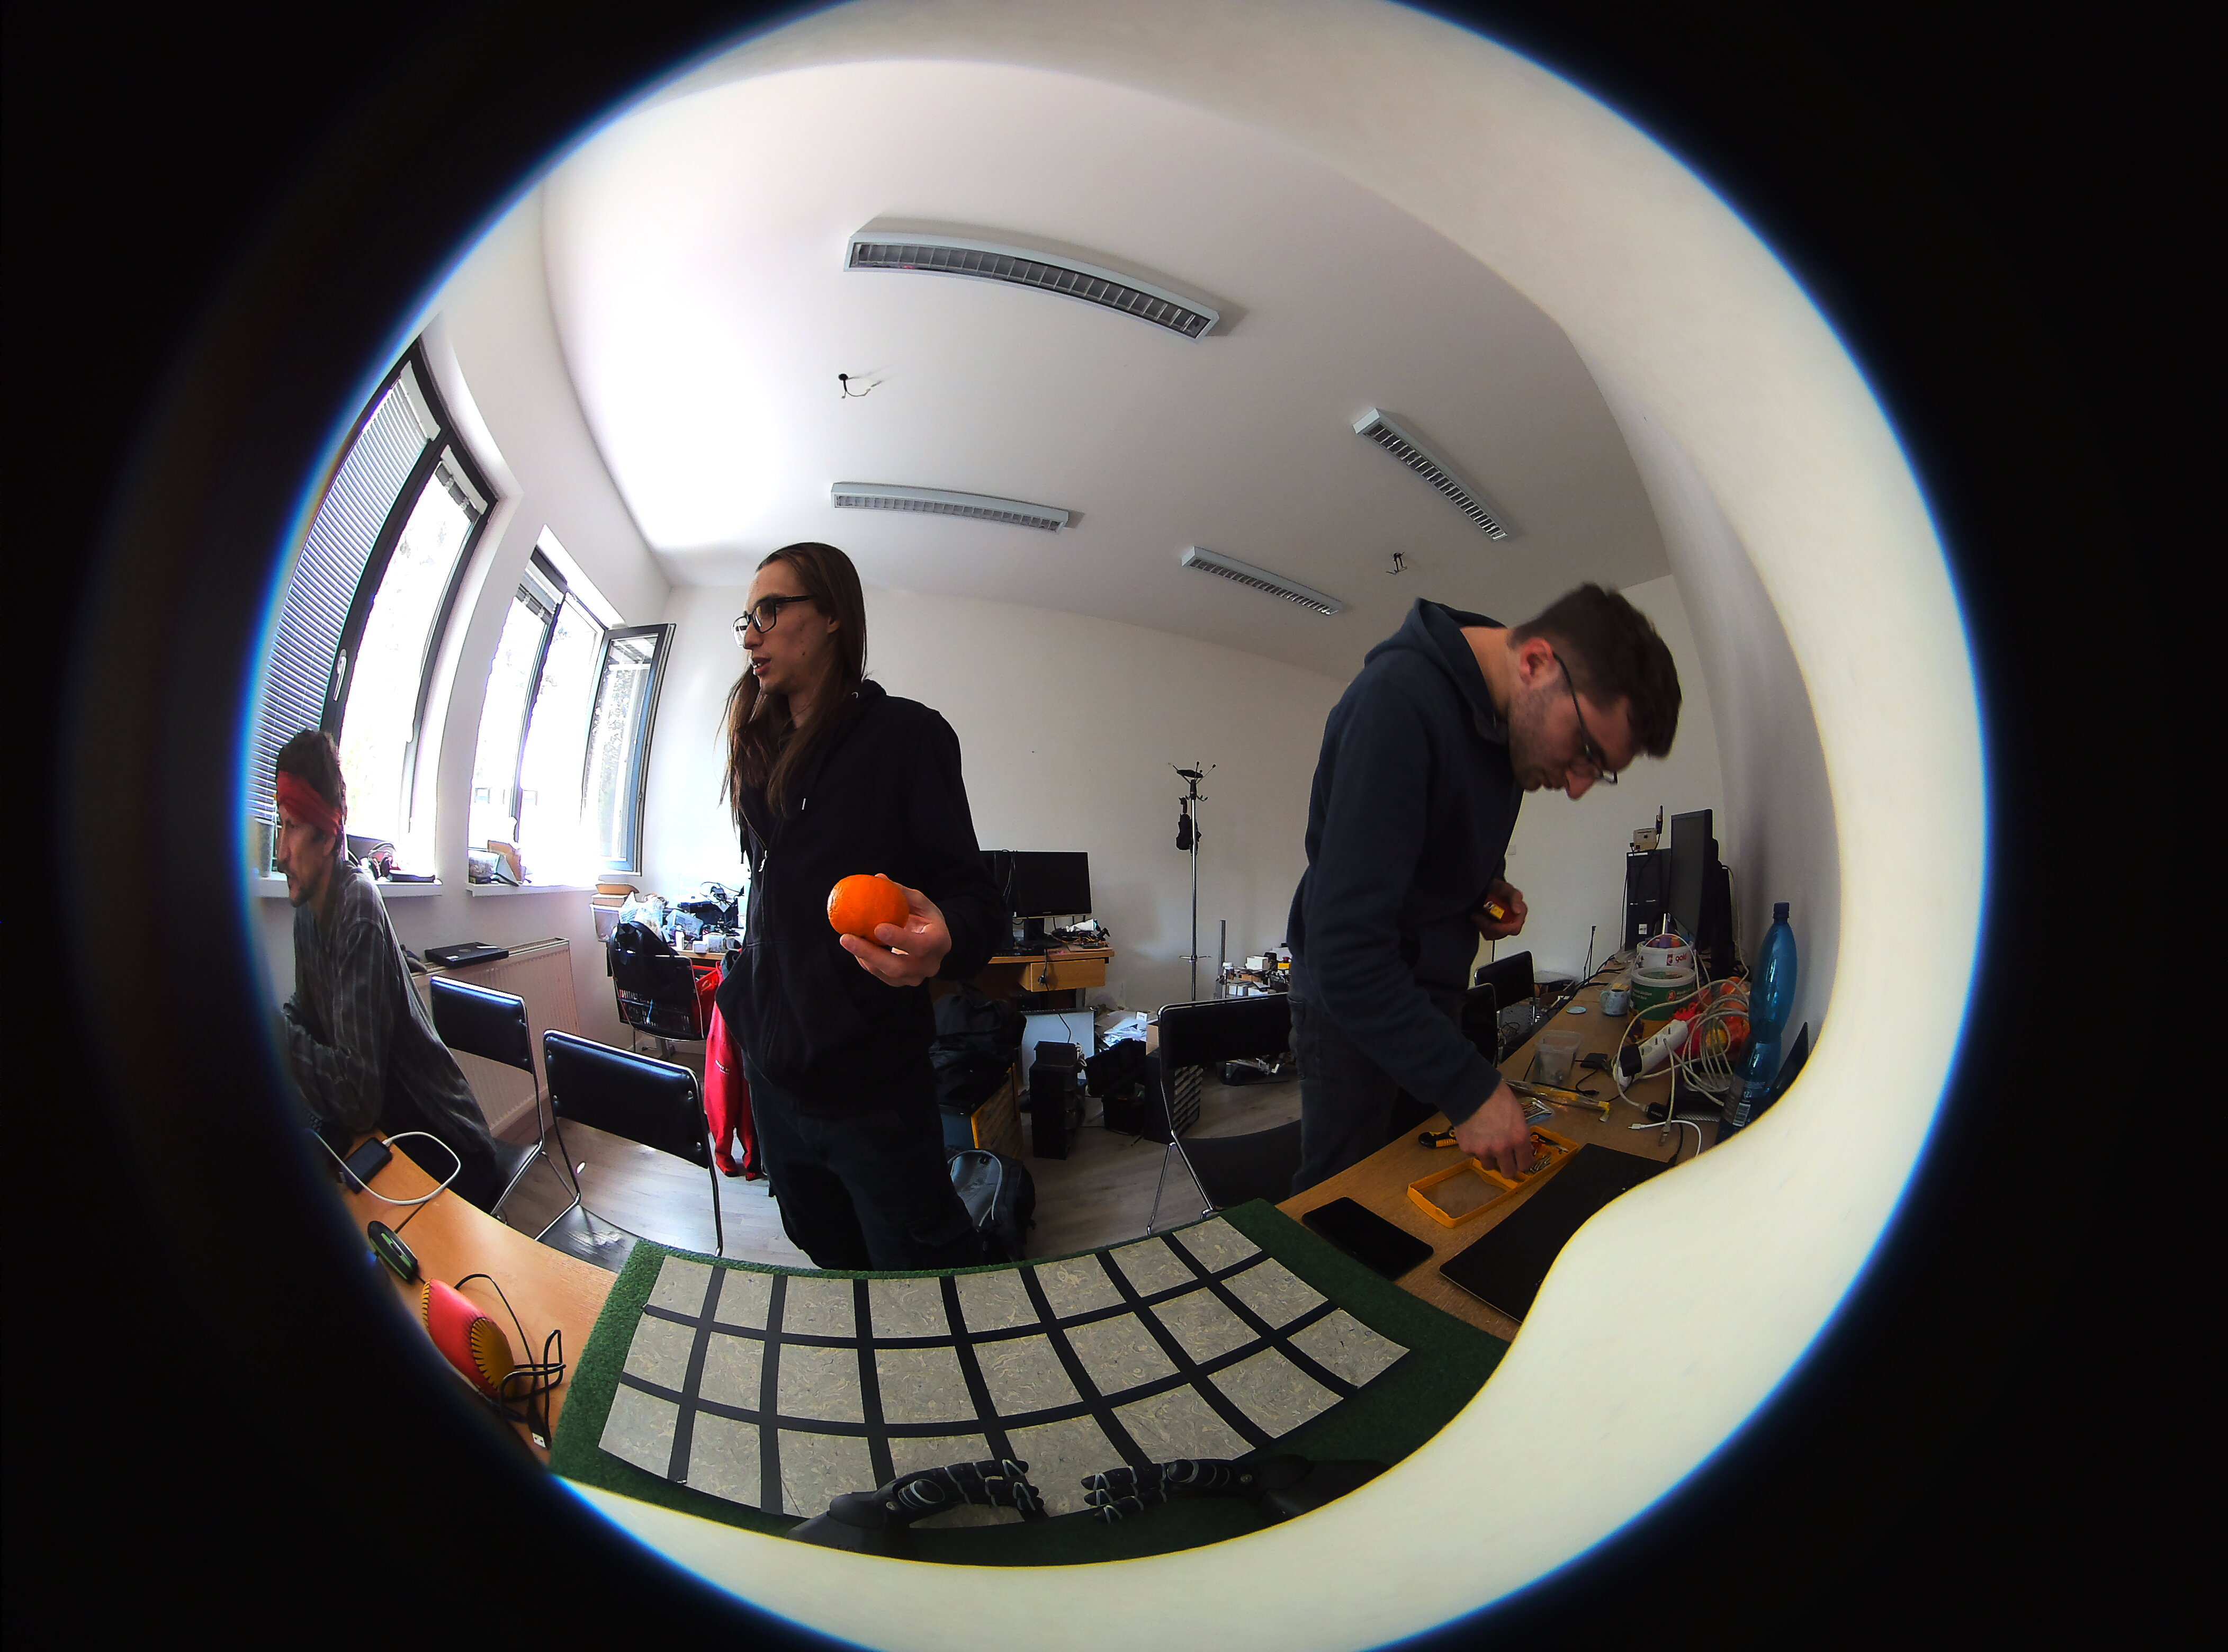
\includegraphics[width=\textwidth]{images/2023-04-17-140320_1.jpg}
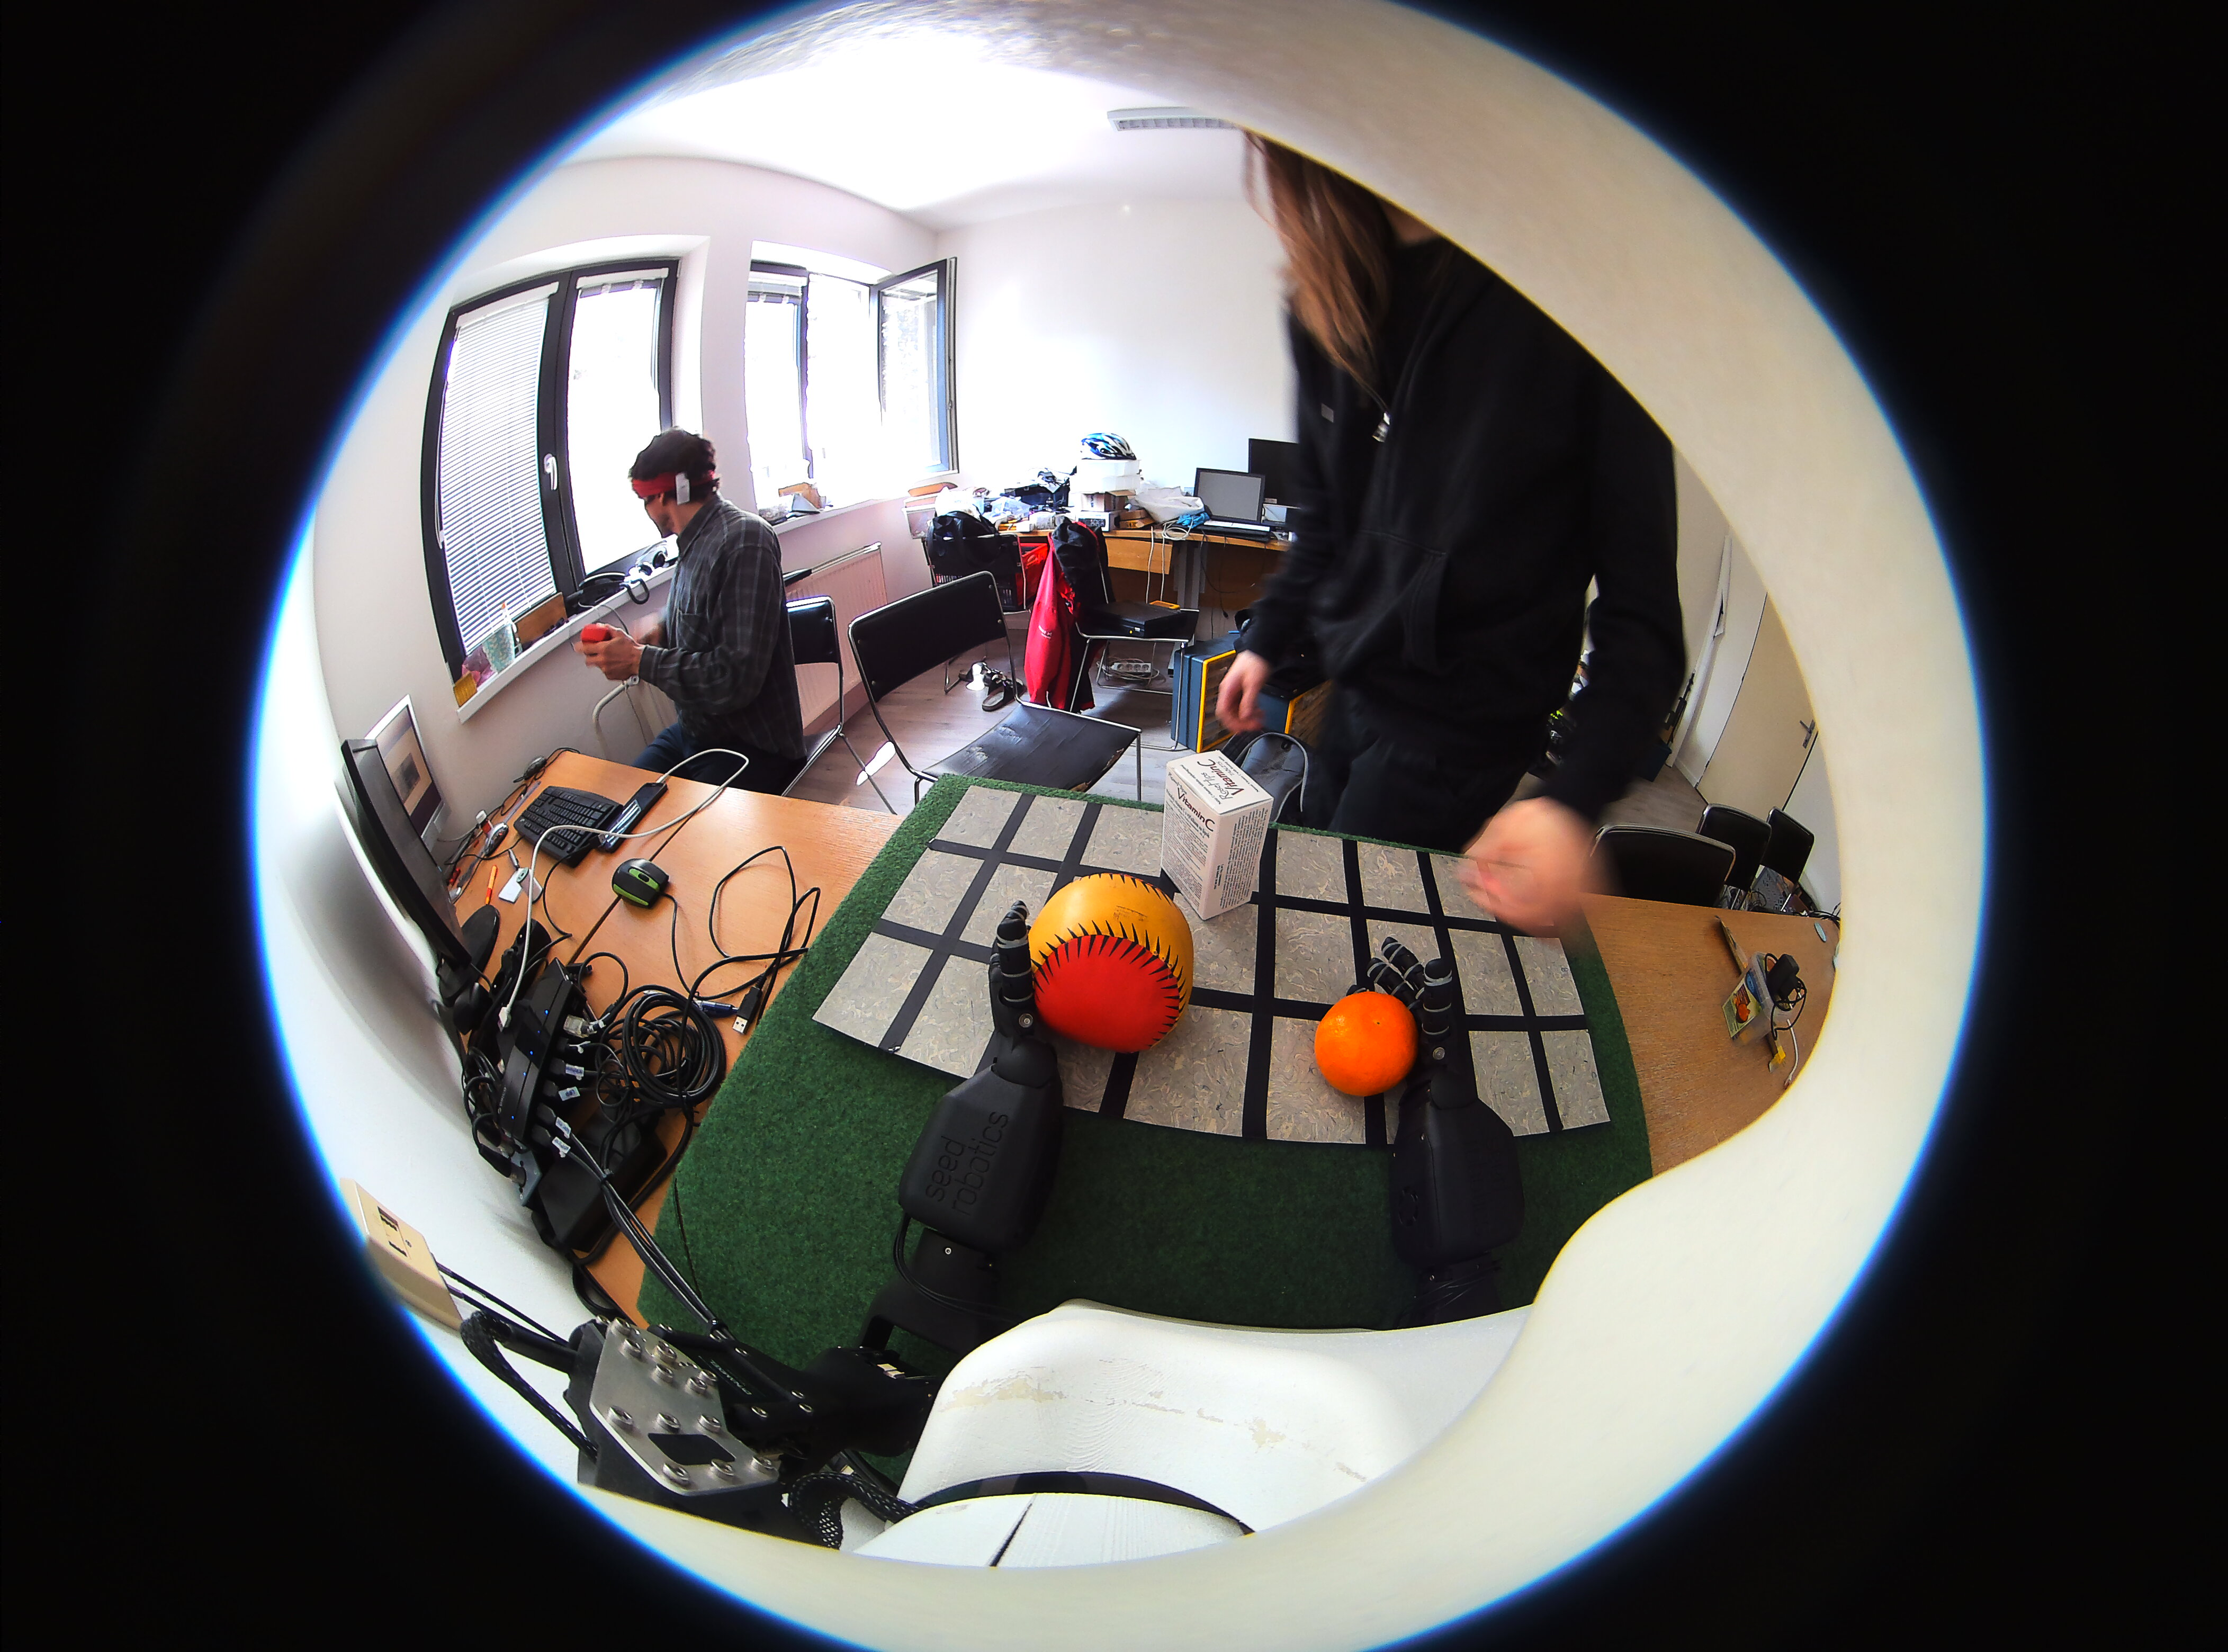
\includegraphics[width=\textwidth]{images/2023-04-17-140935_99.jpg}
\centering
\caption{Príklad trénovacích obrázkov z kamery robota NICO.}
\label{fig:image700}
\end{figure}

\begin{figure}[H]
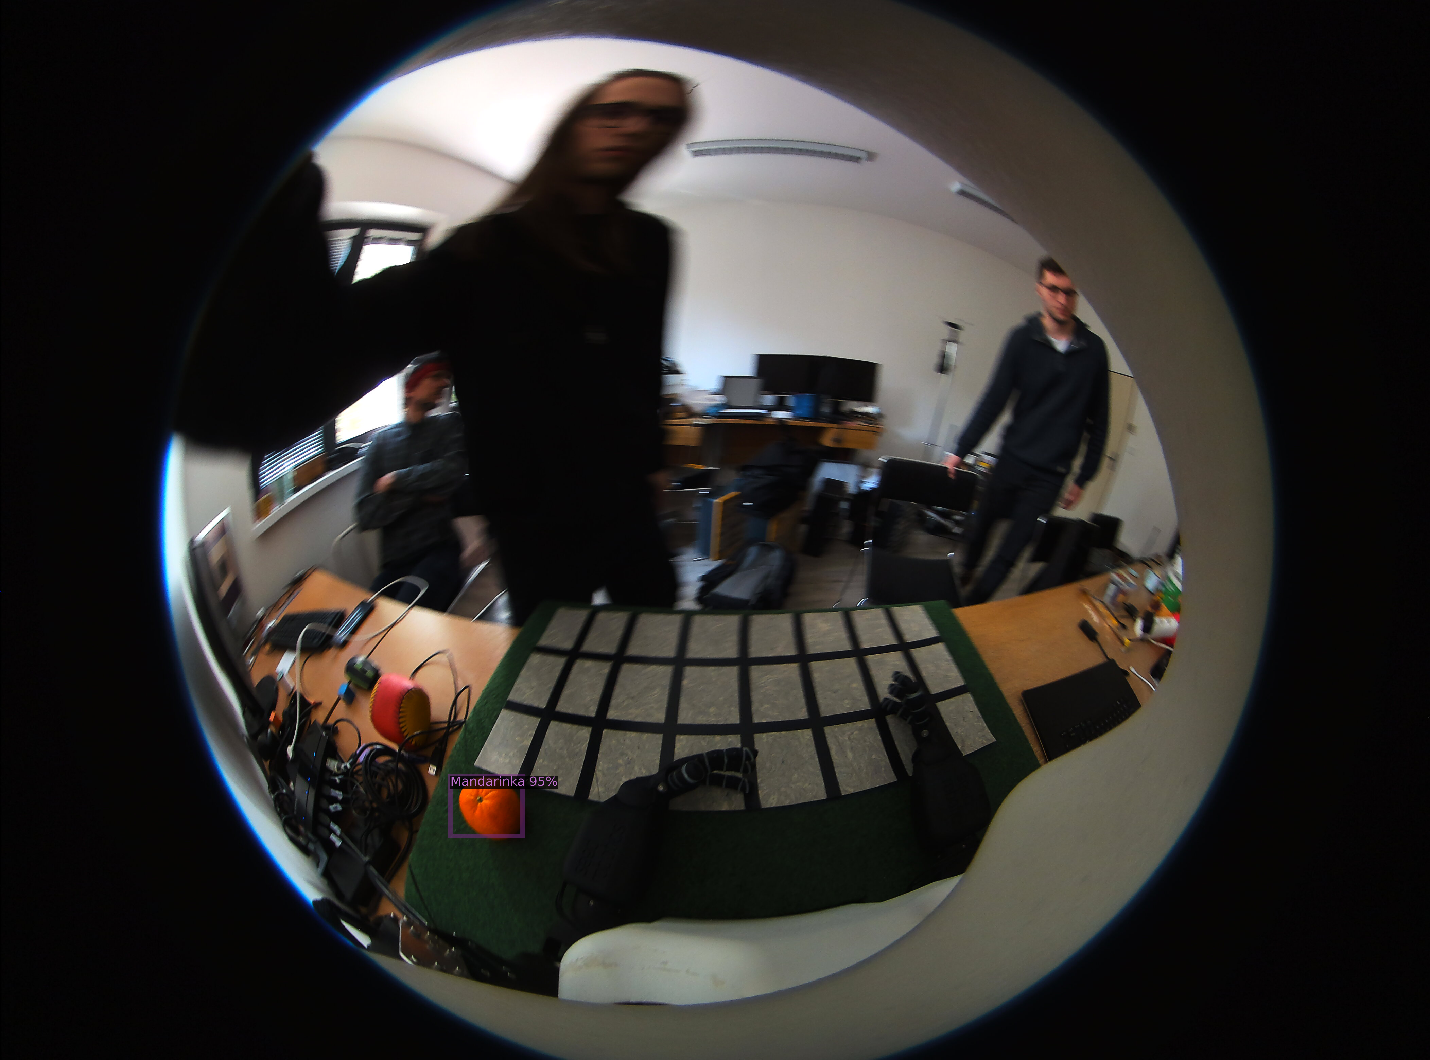
\includegraphics[width=\textwidth]{images/detections_screenshot1.png}
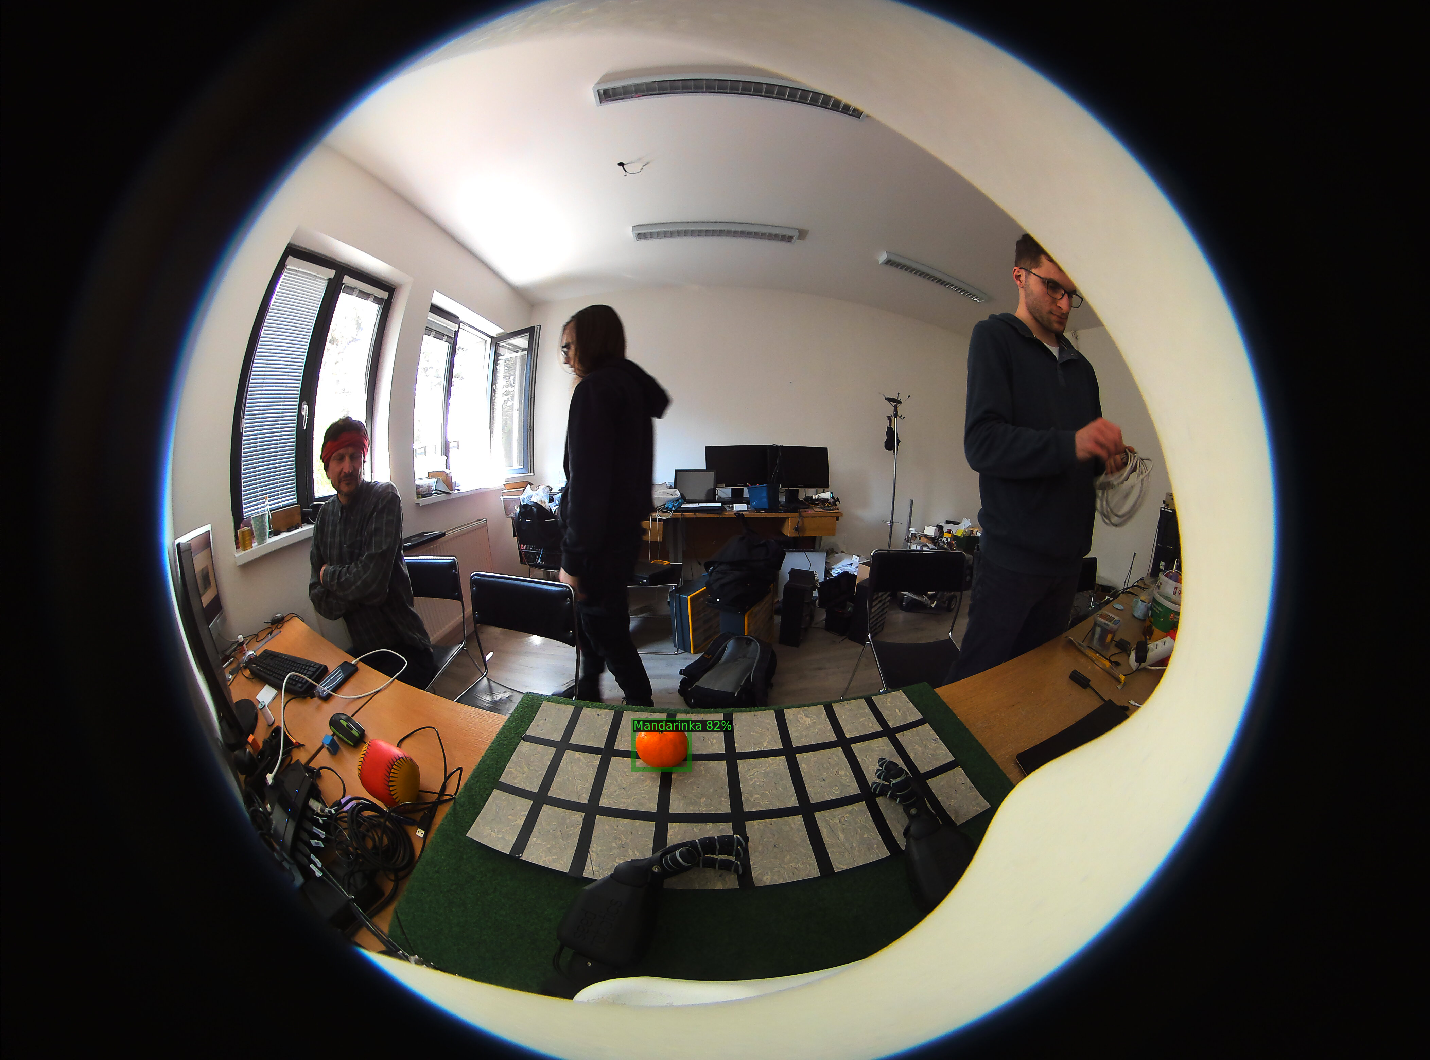
\includegraphics[width=\textwidth]{images/detections_screenshot2.png}
\centering
\caption{Príklad úspešných detekcii testovacích obrázkov z kamery robota NICO.}
\label{fig:image701}
\end{figure}

\begin{figure}[H]
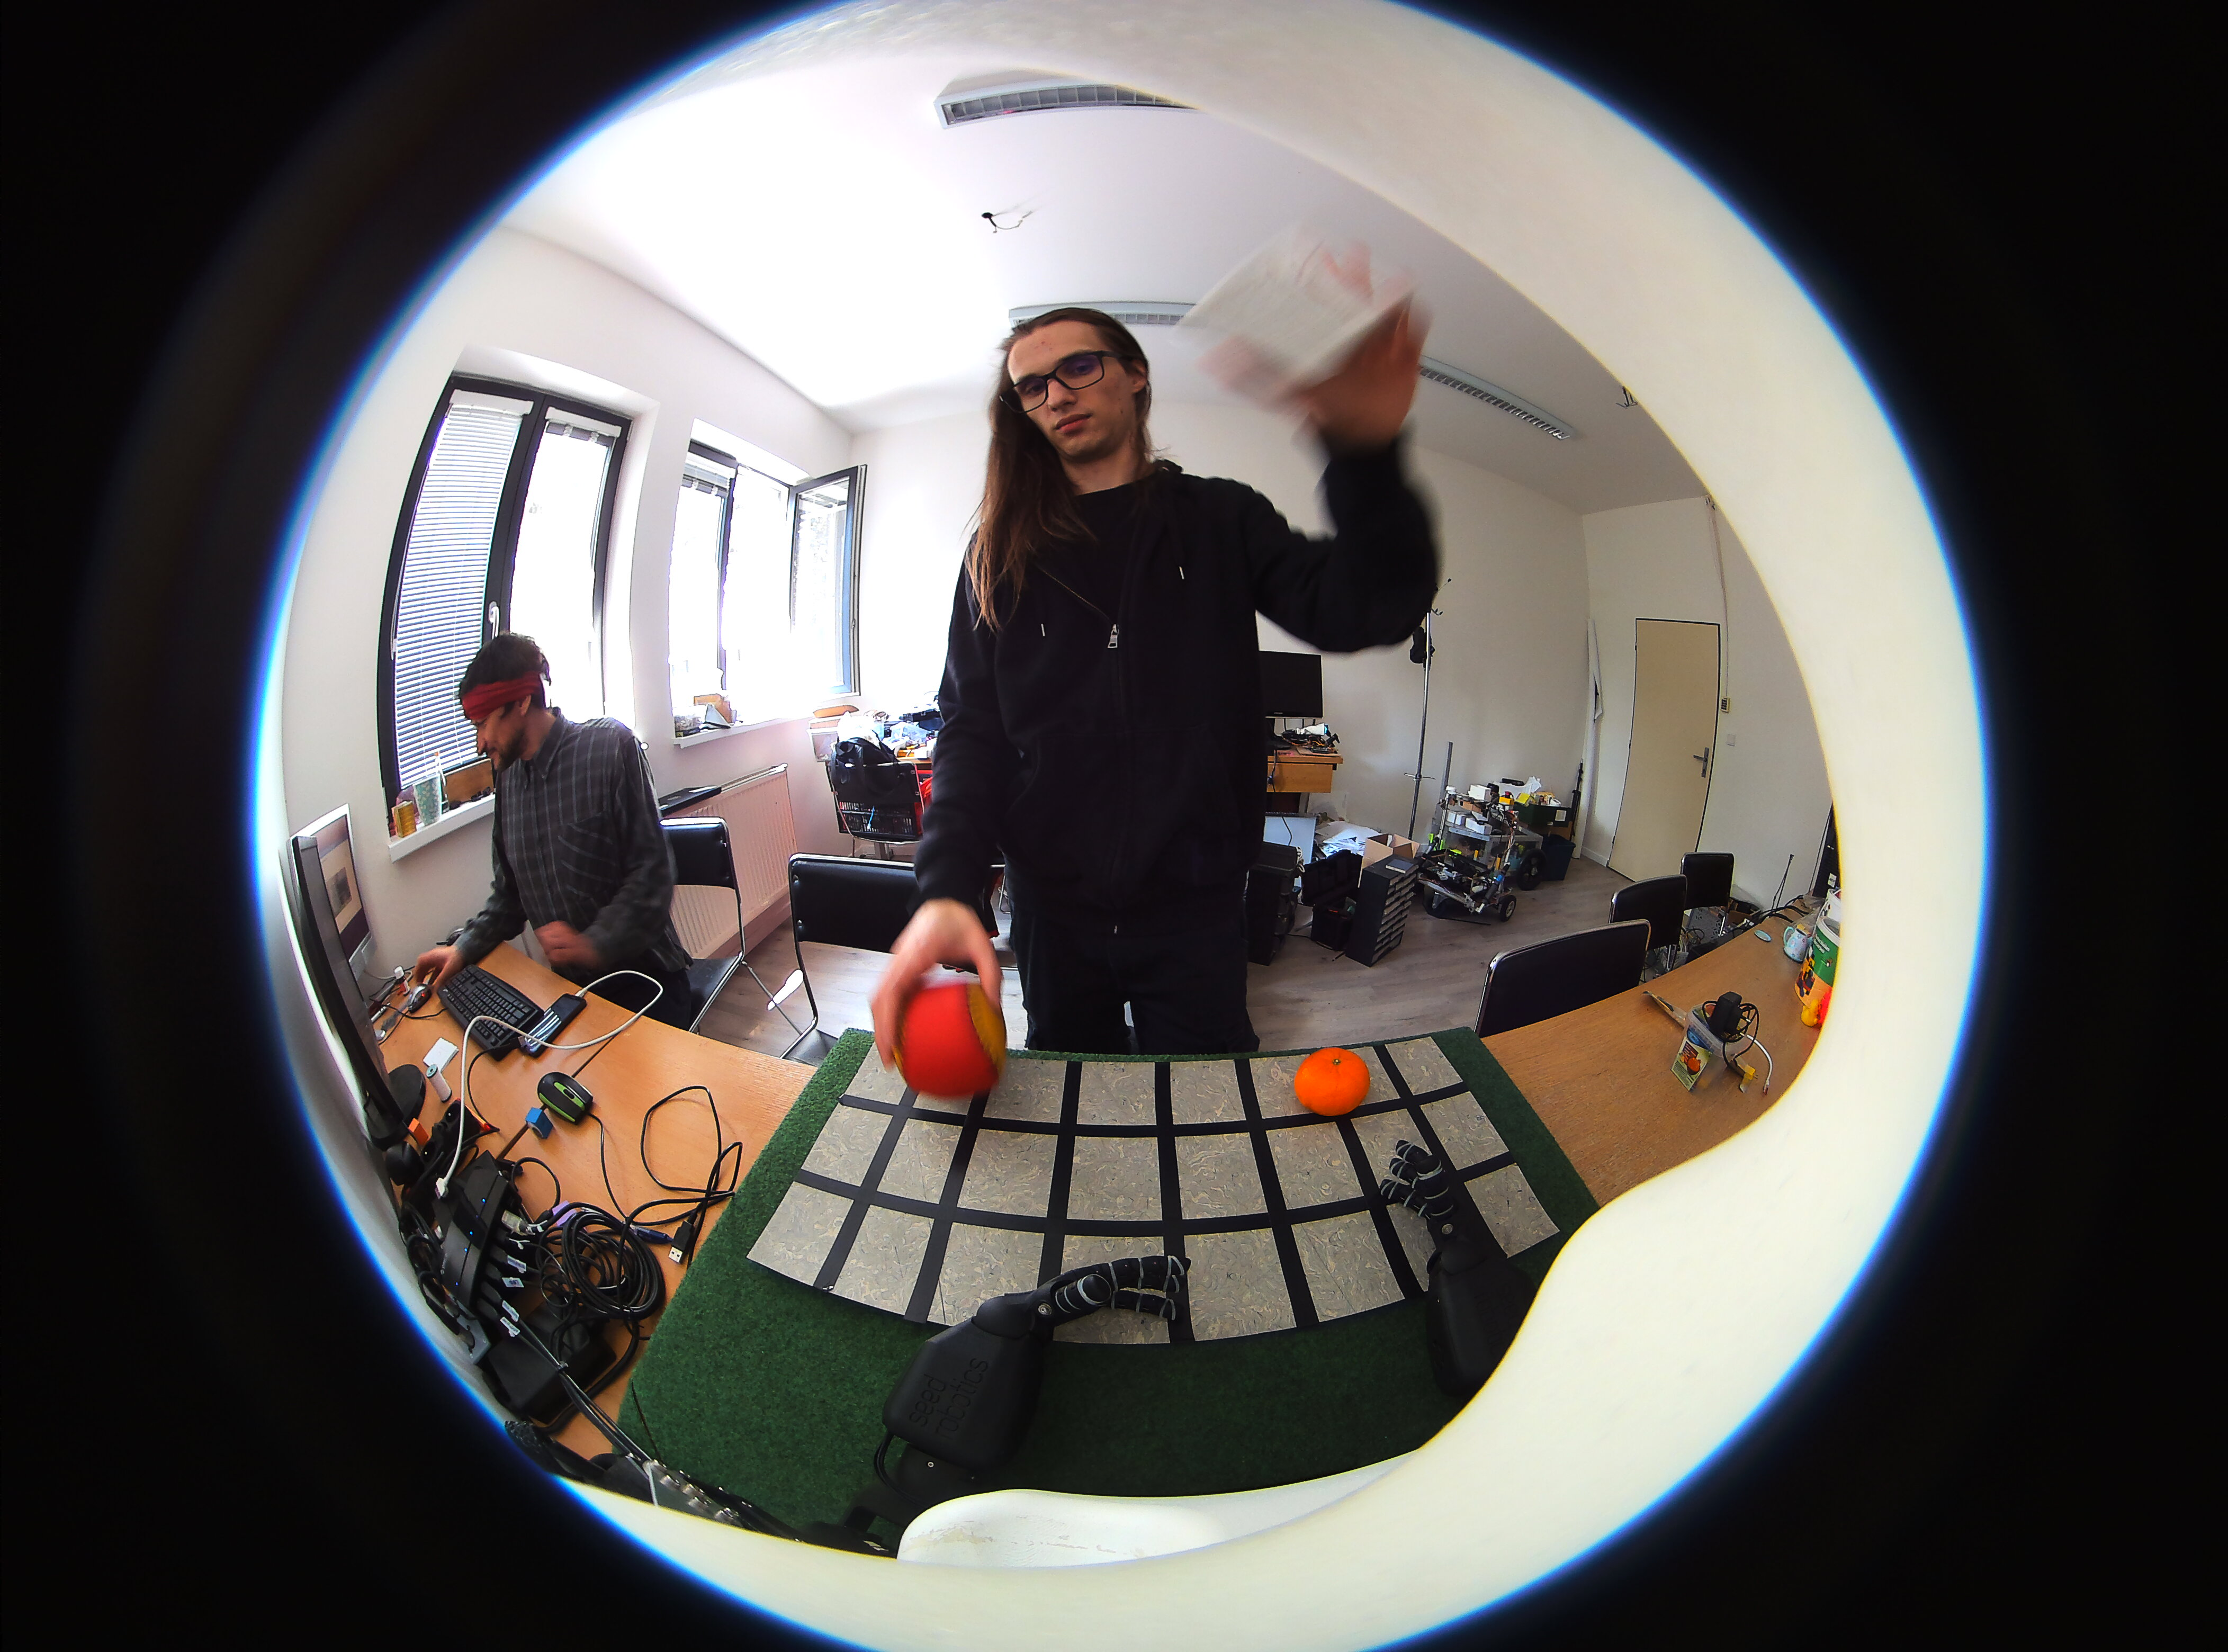
\includegraphics[width=\textwidth]{images/2023-04-17-140935_8.jpg}
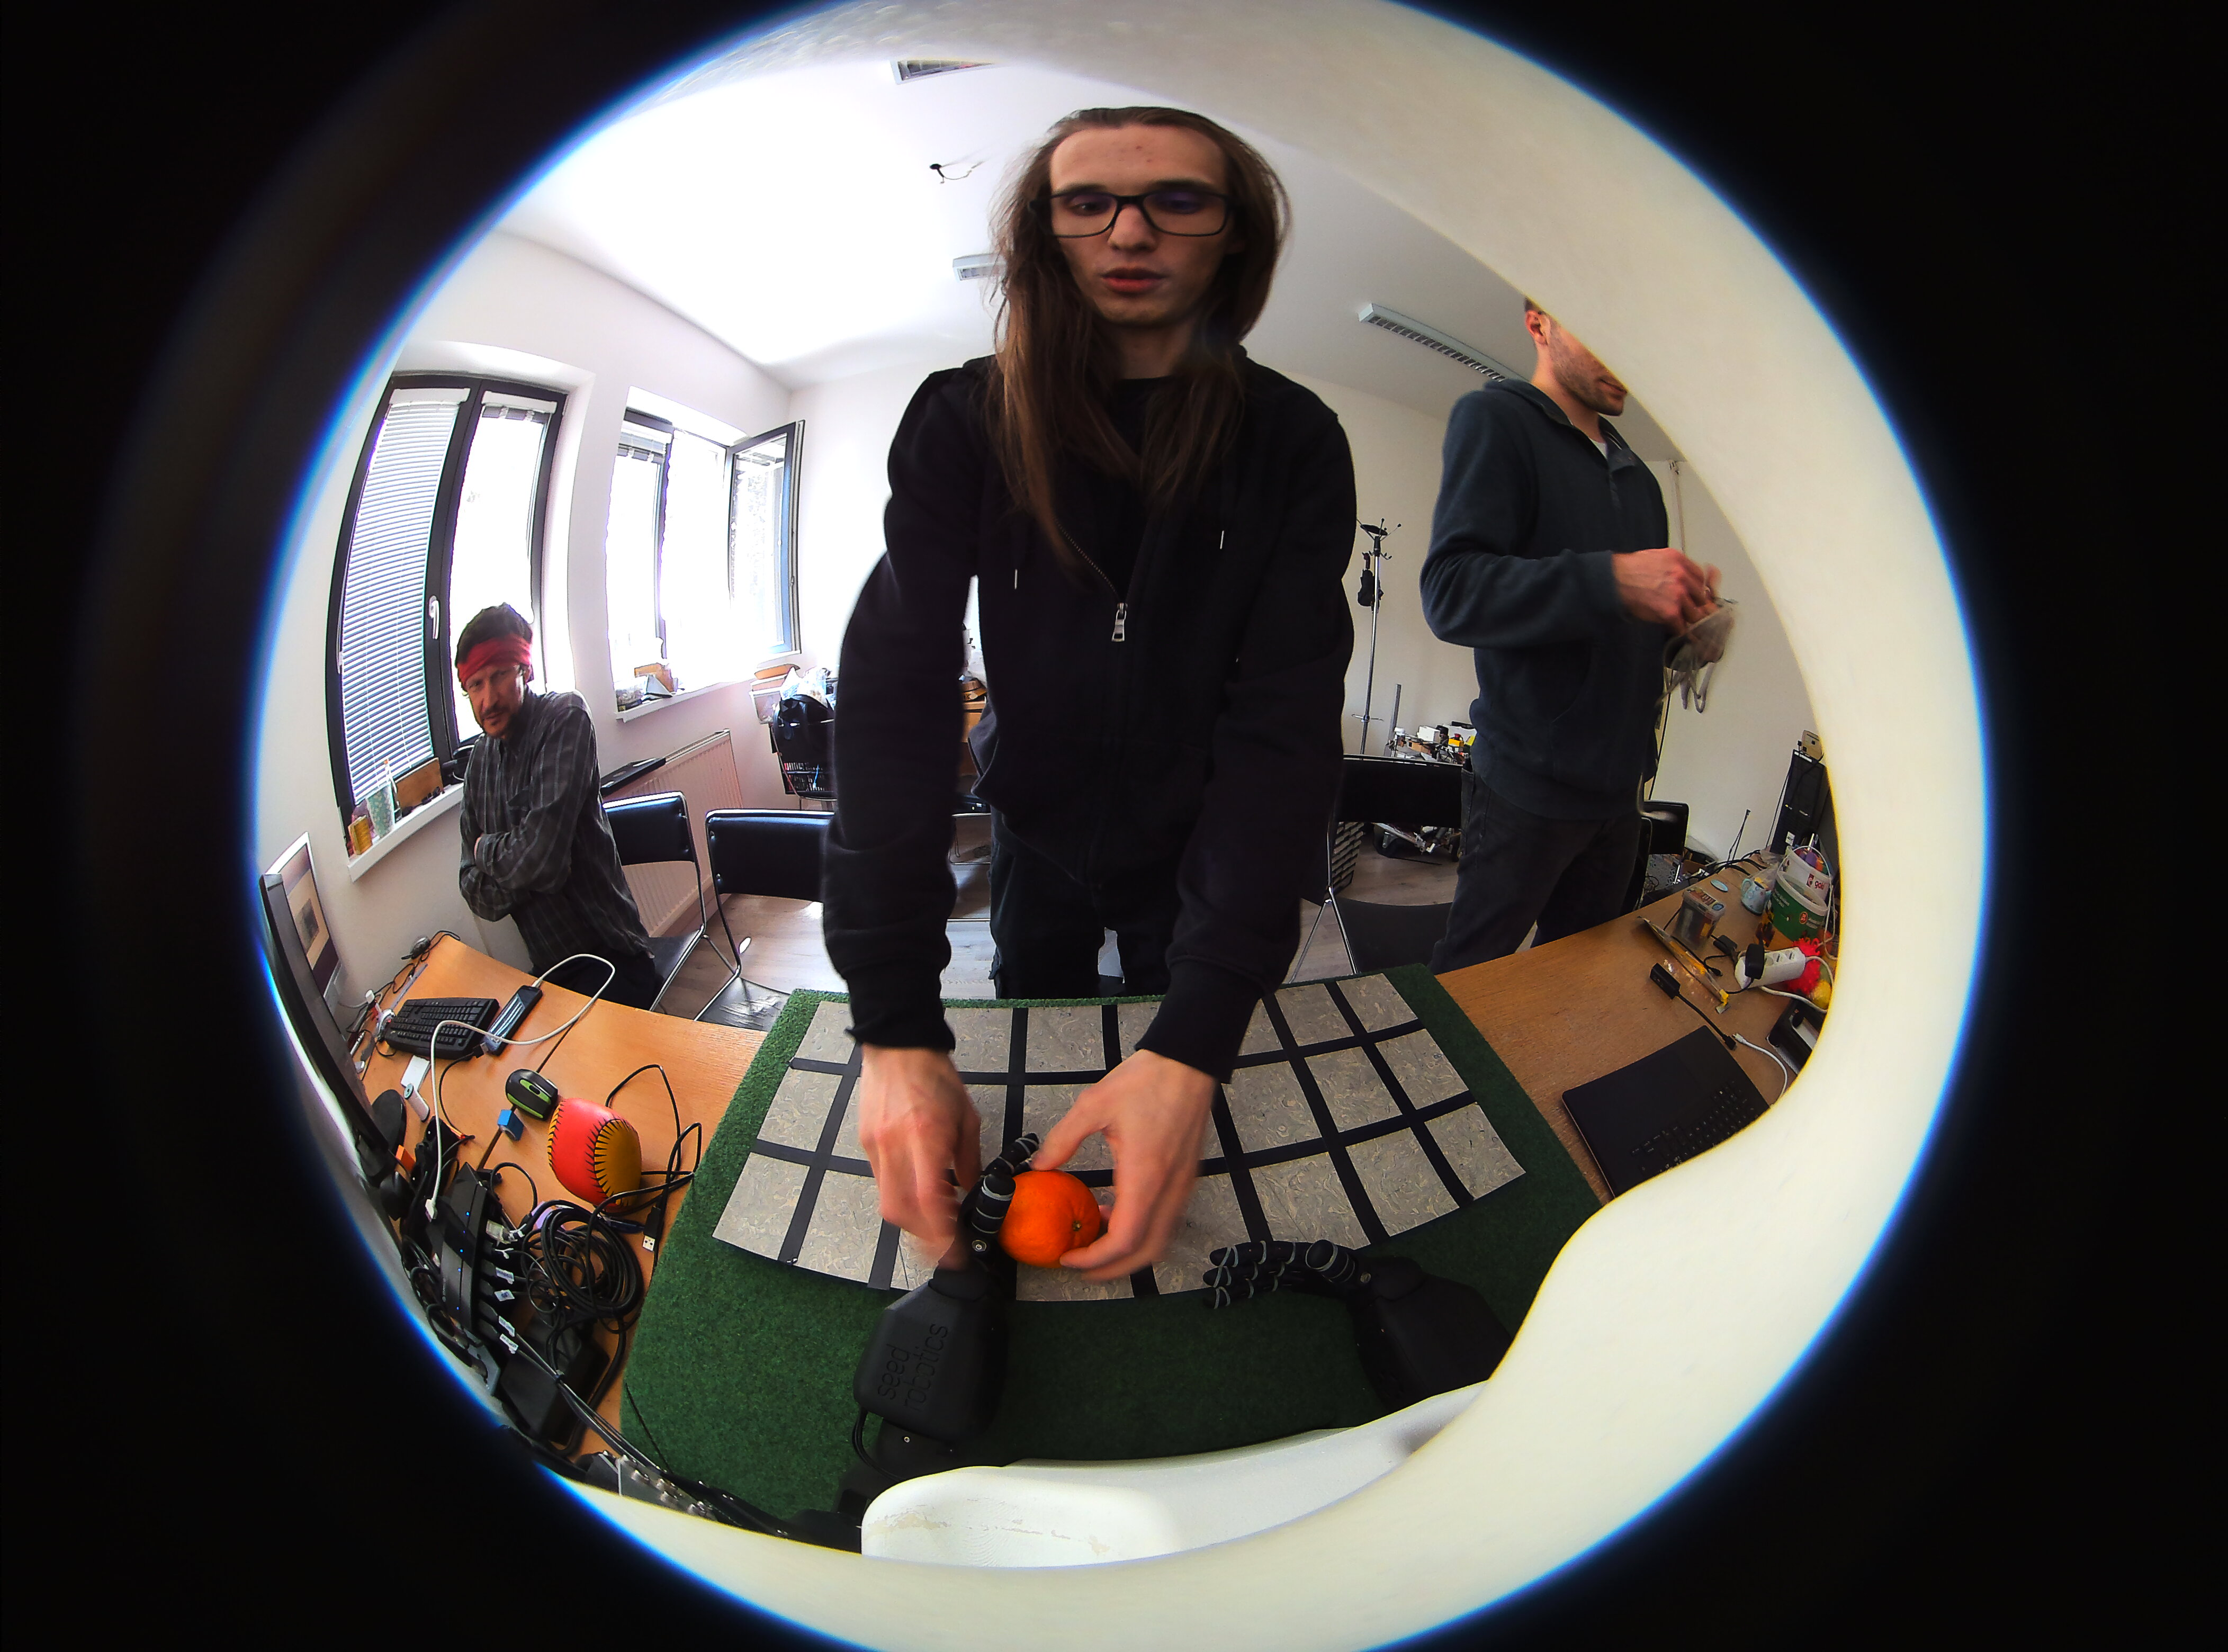
\includegraphics[width=\textwidth]{images/2023-04-17-140334_38.jpg}
\centering
\caption{Príklad neúspešných detekcii testovacích obrázkov z kamery robota NICO.}
\label{fig:image702}
\end{figure}

\begin{table}[H]
\begin{tabular}{|l|c|c|c|}
\hline
\textbf{Trieda} & \textbf{mAP} & \textbf{AP50} & \textbf{AP75} \\
\hline
Mandarinka & 14.545 & 18.182 & 18.182 \\
\hline
\end{tabular}
\centering
\caption{Tabuľka presností na testovacích dátach pri detekcií mandarinky pomocou snímok z kamery robota NICO.}
\label{tab:table700}
\end{table}

\begin{table}[H]
\begin{tabular}{|l|c|c|c|c|}
\hline
\textbf{Trieda} & \textbf{Počet obrázkov} & \textbf{Úspešné} & \textbf{Neúspešné} &  \textbf{Nedetegované}\\
\hline
Mandarinka & 30 & 4 & 0 & 26 \\
\hline
\end{tabular}
\centering
\caption{Tabuľka jednoduchšej presnosti na testovacích dátach pri detekcií mandarinky pomocou snímok z kamery robota NICO pri confidence threshold = 0.5.}
\label{tab:table702}
\end{table}

\section{Testovanie na snímkoch z kamery zbavených skreslenia}

Ako vidíme naša presnosť, nie je príliš vysoká, za čo zrejmä môže aj nižšia kvalita našich obrázkov. Teraz vyskúšame natrénovať a vyhodnotiť model na obrázkoch bez skreslenia. Na zbavenia sa skreslenia použijeme knižnicu \texttt{planar\_nico\_vision} \cite{planarNicoVision}. Po odstránení skreslenia, sme na niektorých obrázkoch odrezali taktiež mandarinku. Takže sa náš dataset kvalitných obrázkov zredukoval na 30. Rozdelíme teda dataset na 10 trénovacích a 20 testovacích obrázkov. 

Na obrázku \ref{fig:image703} vidíme príklady trénovacích obrázkov, na obrázku \ref{fig:image704} vidíme príklady úspešných detekcií na testovacích obrázkoch, na obrázku \ref{fig:image705} vidíme príklady neúspešných detekcií na testovacích obrázkoch, v tabuľke \ref{tab:table701} vidíme výslednú presnosť nášho modelu a v tabuľke \ref{tab:table703} vidíme jednoduchšiu presnosť nášho modelu pre lepšiu interpretáciu, pri confidence threshold = 0.1. Naša presnosť bola taká nízka, že sme museli zížiť confidence threshold aby sme dostali aspoň nejaké správne detekcie.

Vidíme, že zbavenie skreslenia nám nepomohlo a dosahujeme ešte nižšiu presnosť ako z pôvodných, neupravených snimkov. 

\begin{figure}[H]
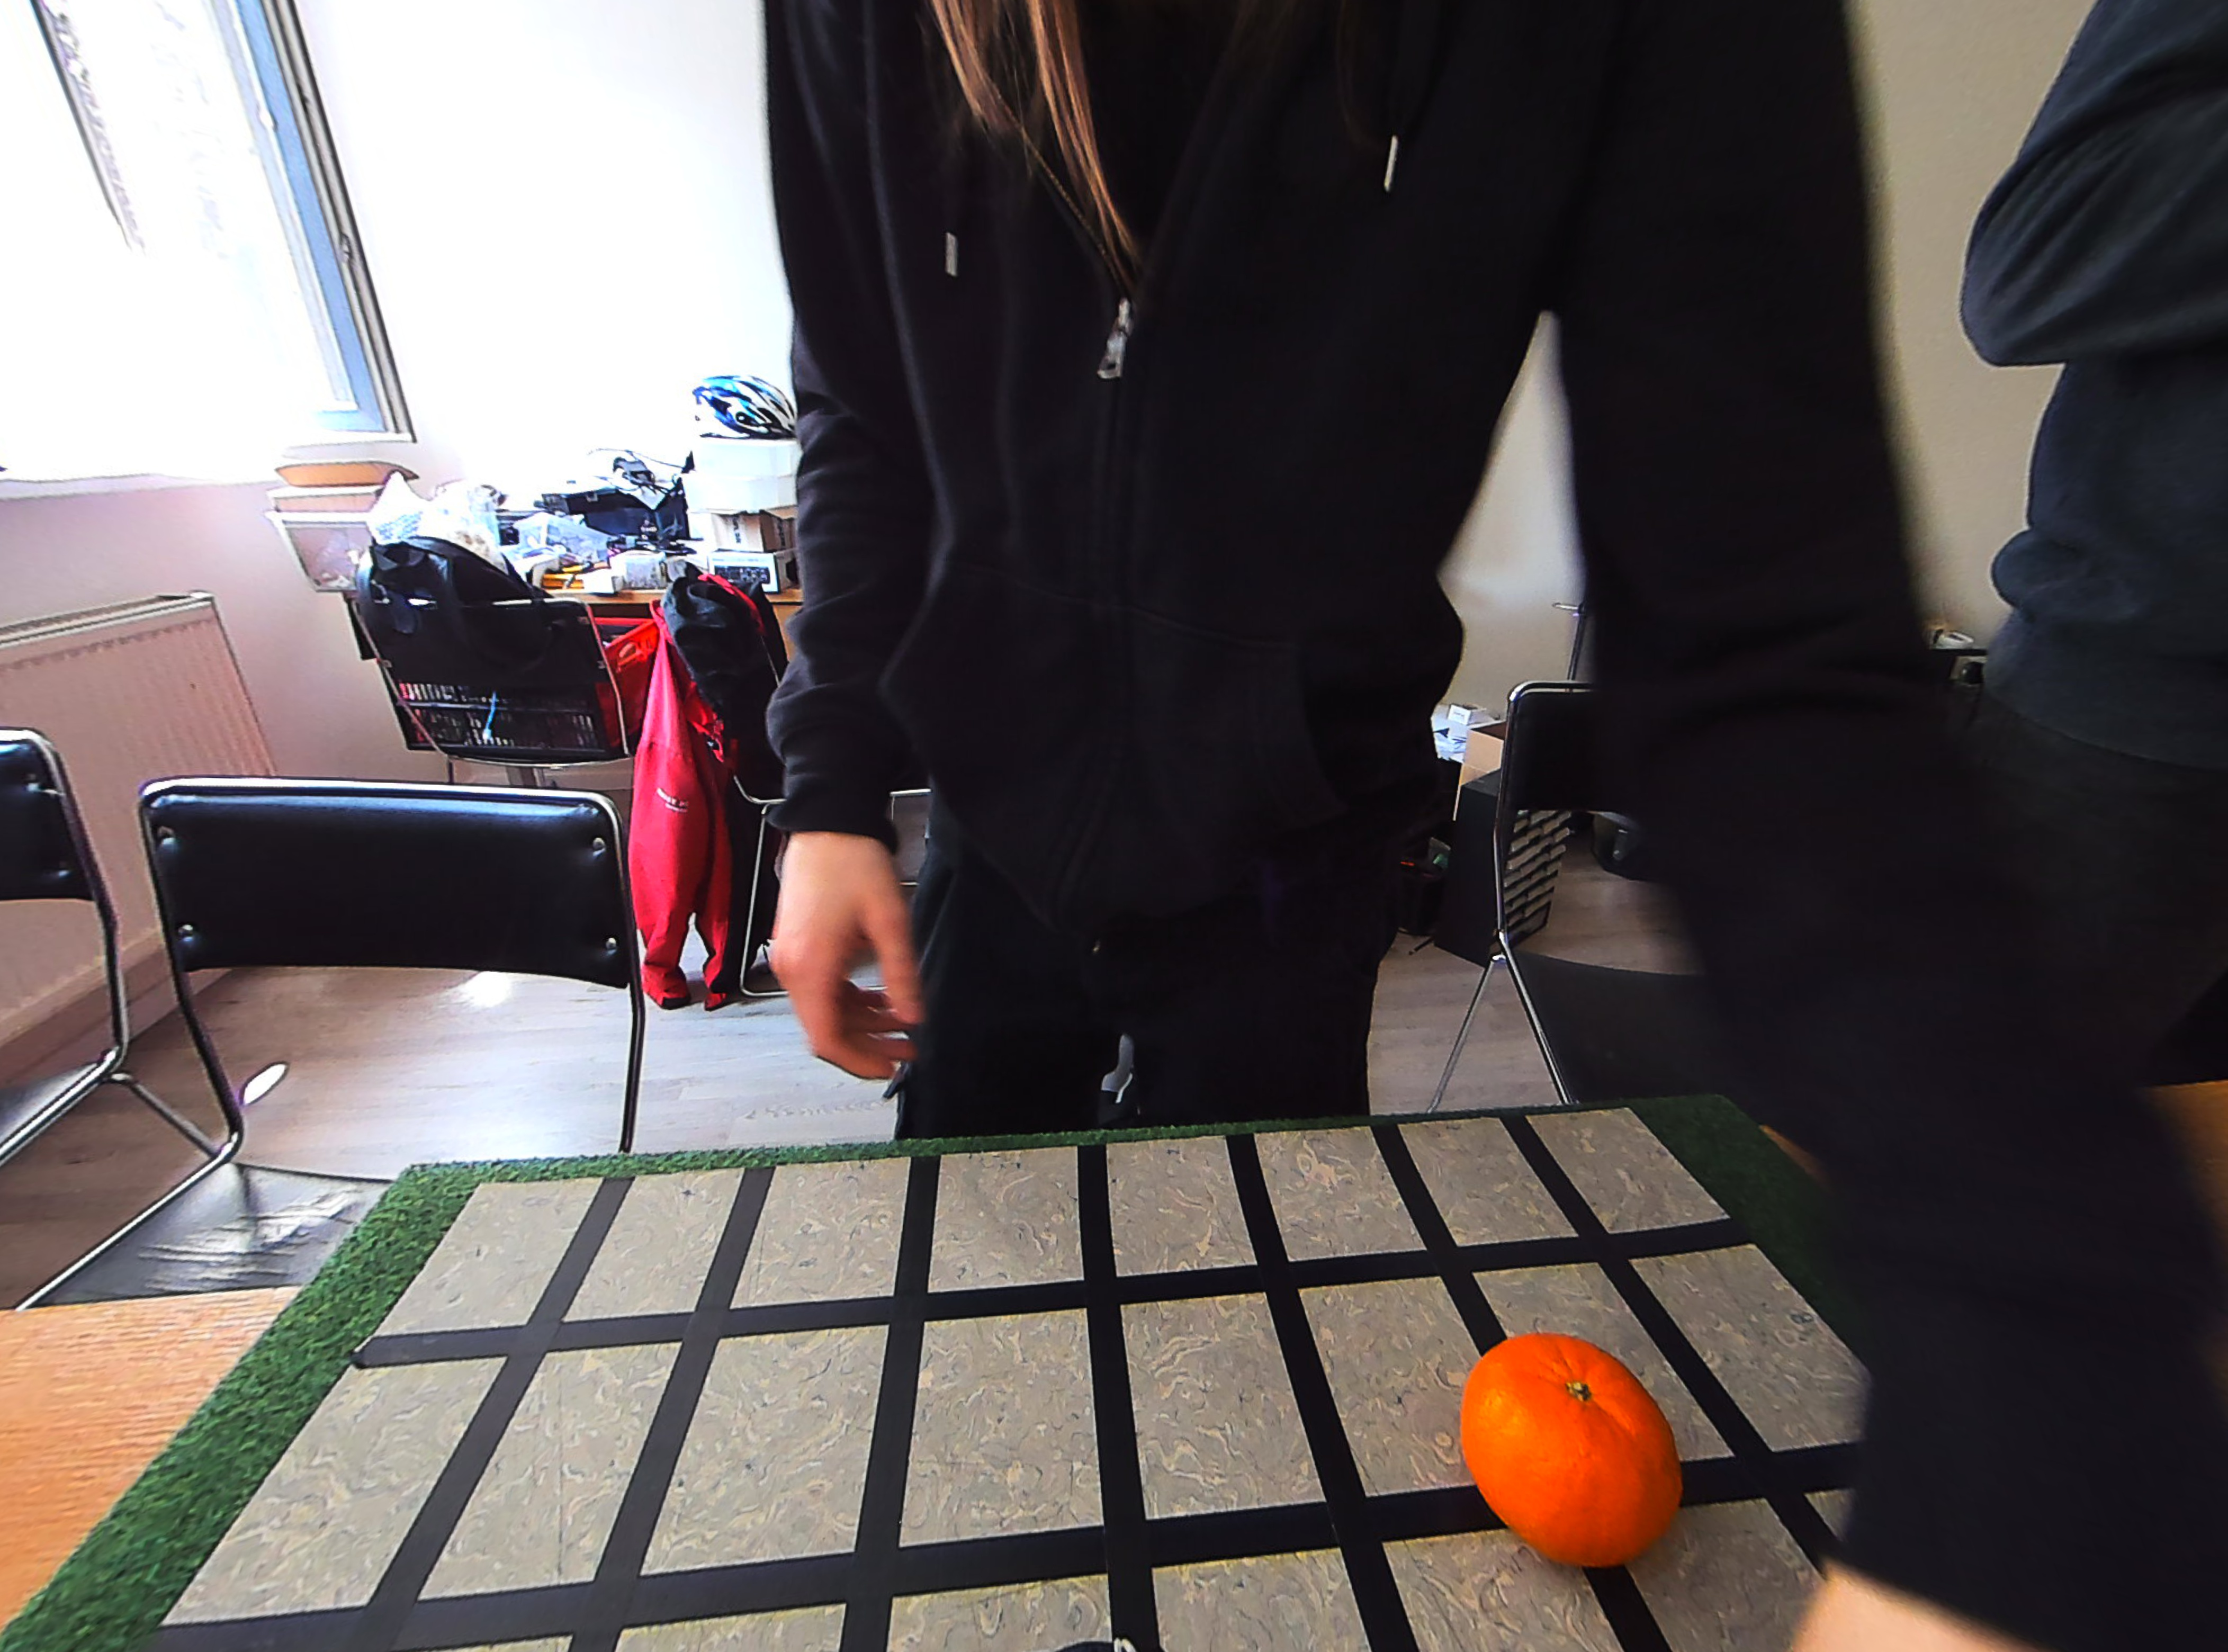
\includegraphics[width=\textwidth]{images/2023-04-17-140334_41_clean.jpg}
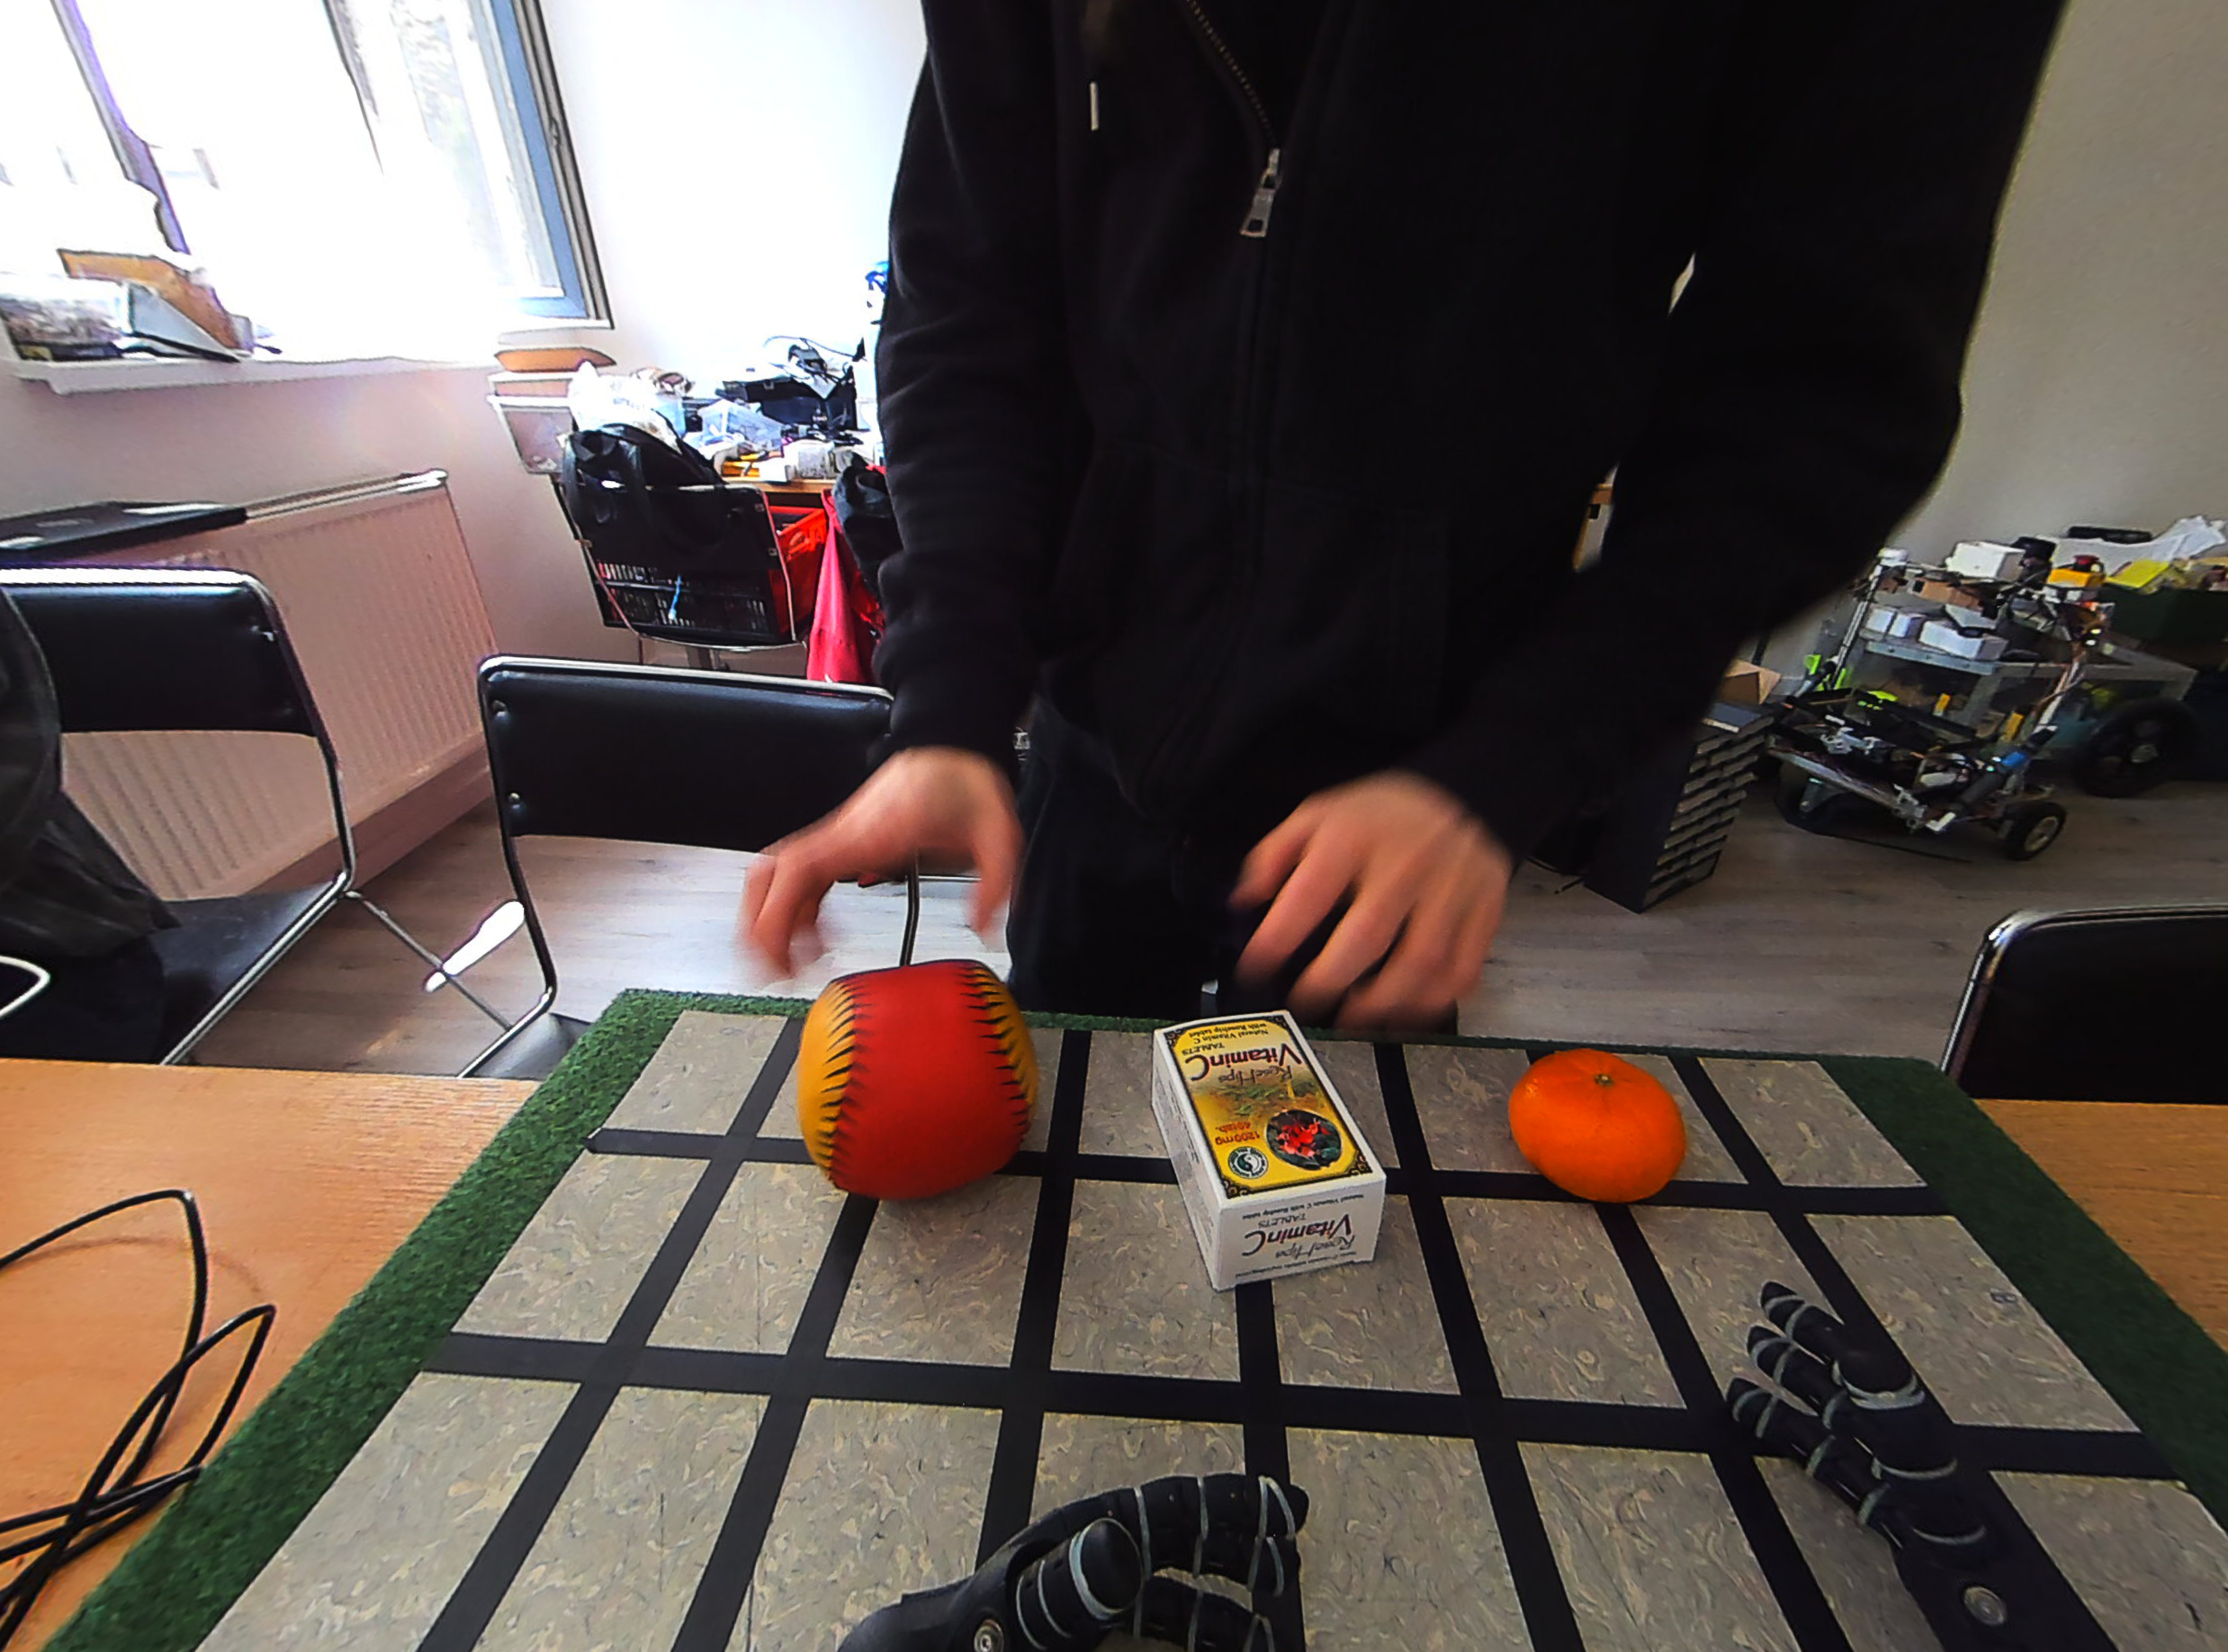
\includegraphics[width=\textwidth]{images/2023-04-17-140935_2_clean.jpg}
\centering
\caption{Príklad trénovacích obrázkov z kamery robota NICO zbavených skreslenia.}
\label{fig:image703}
\end{figure}

\begin{figure}[H]
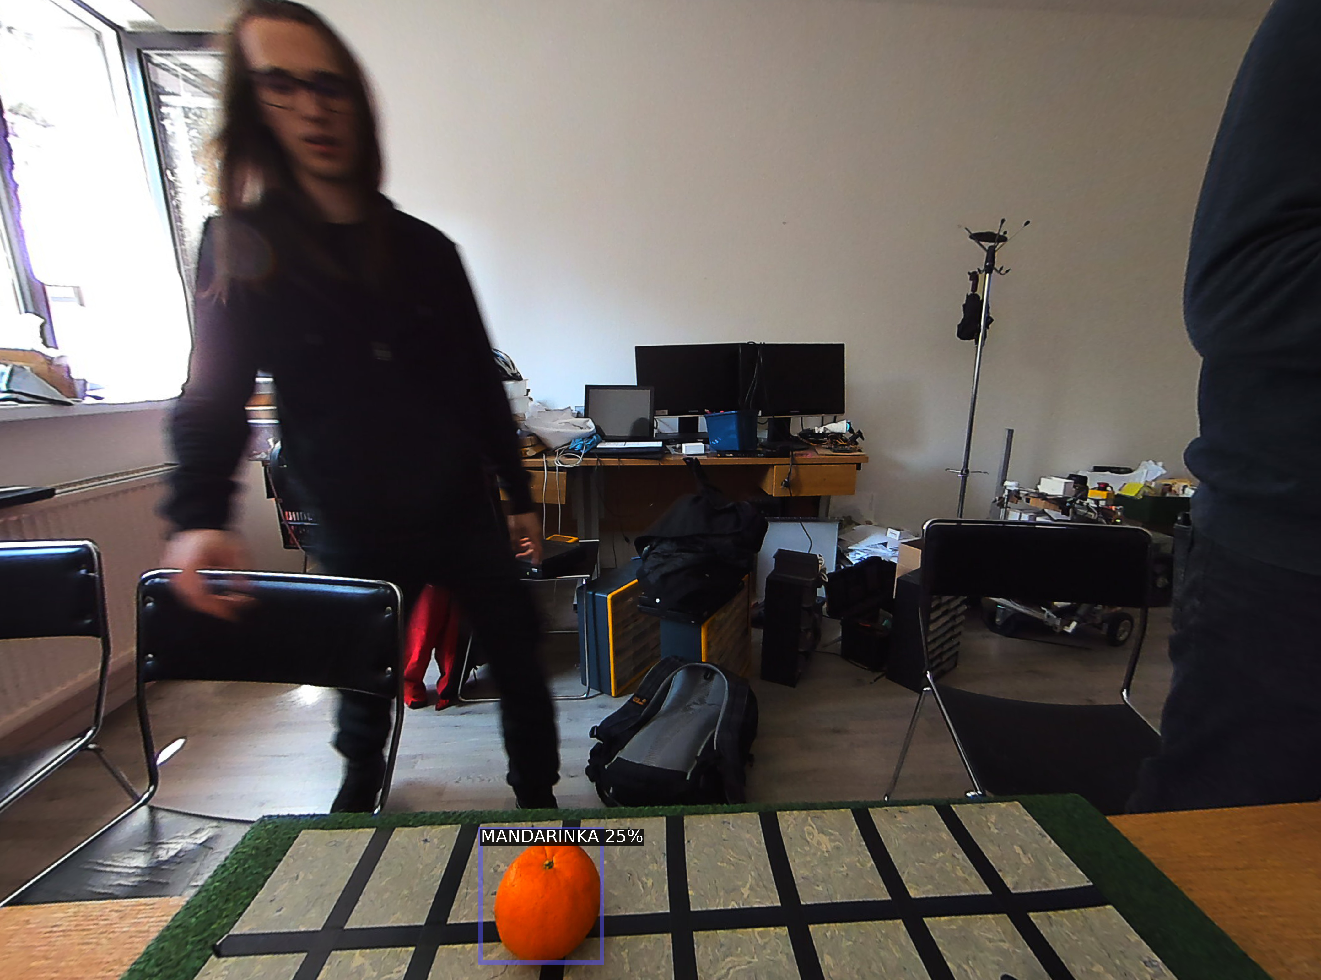
\includegraphics[width=\textwidth]{images/detections_screenshot_clean1.png}
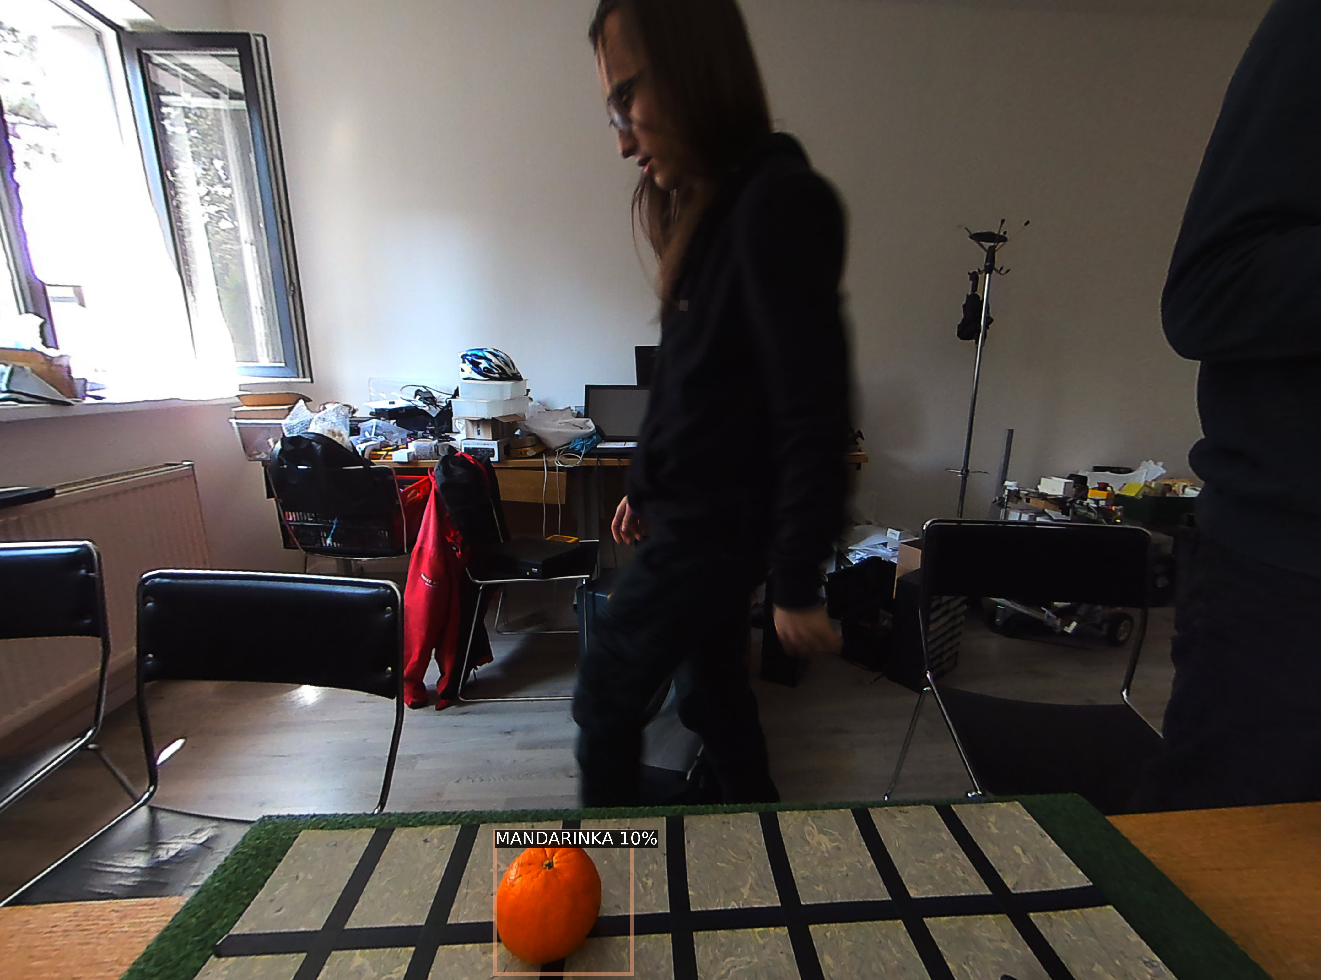
\includegraphics[width=\textwidth]{images/detections_screenshot_clean2.png}
\centering
\caption{Príklad úspešných detekcii testovacích obrázkov z kamery robota NICO zbavených skreslenia.}
\label{fig:image704}
\end{figure}

\begin{figure}[H]
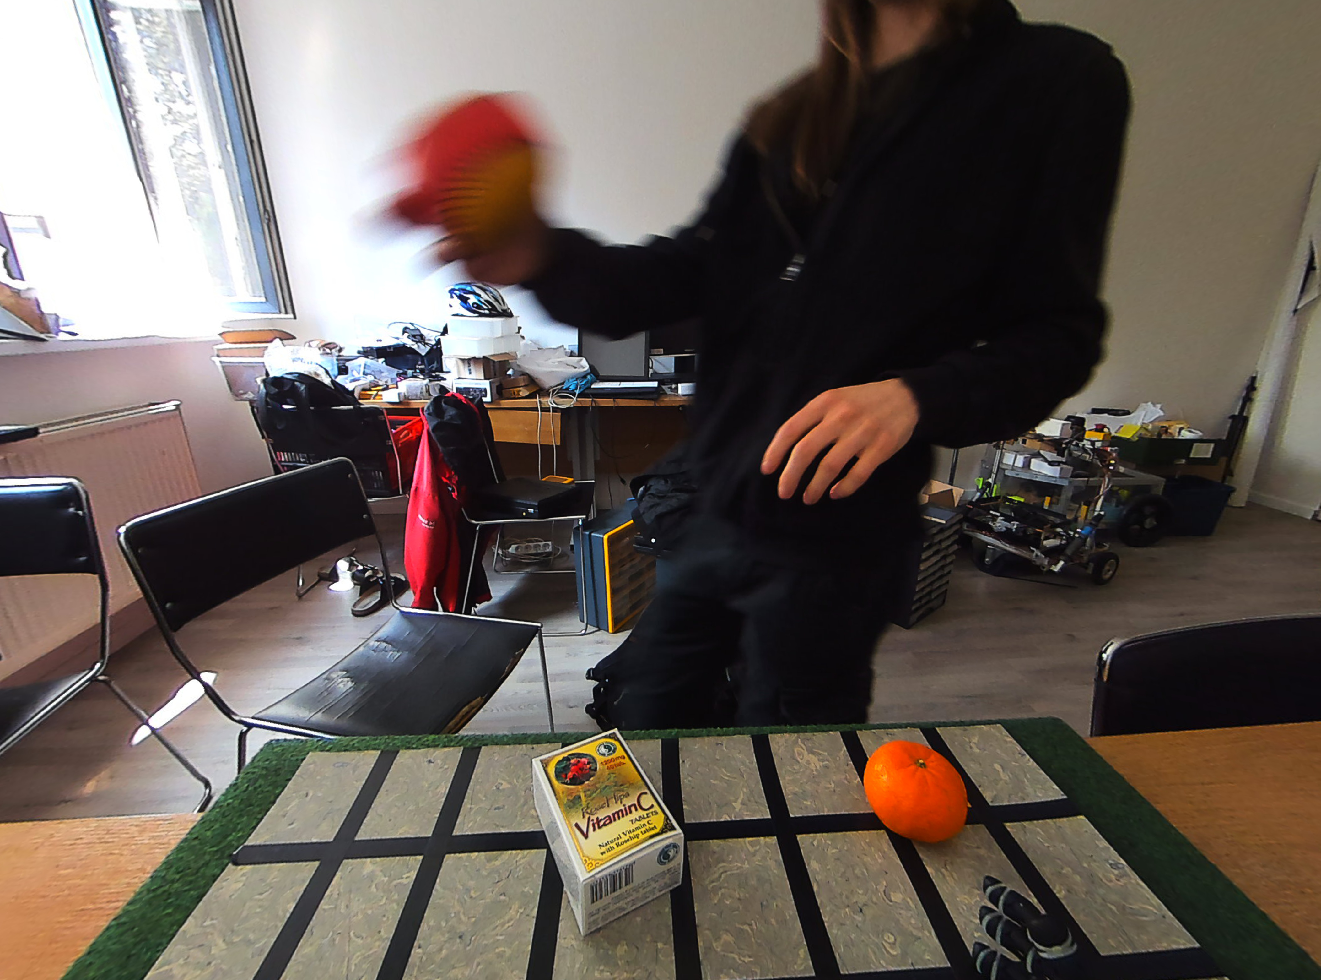
\includegraphics[width=\textwidth]{images/detections_screenshot_clean_wrong1.png}
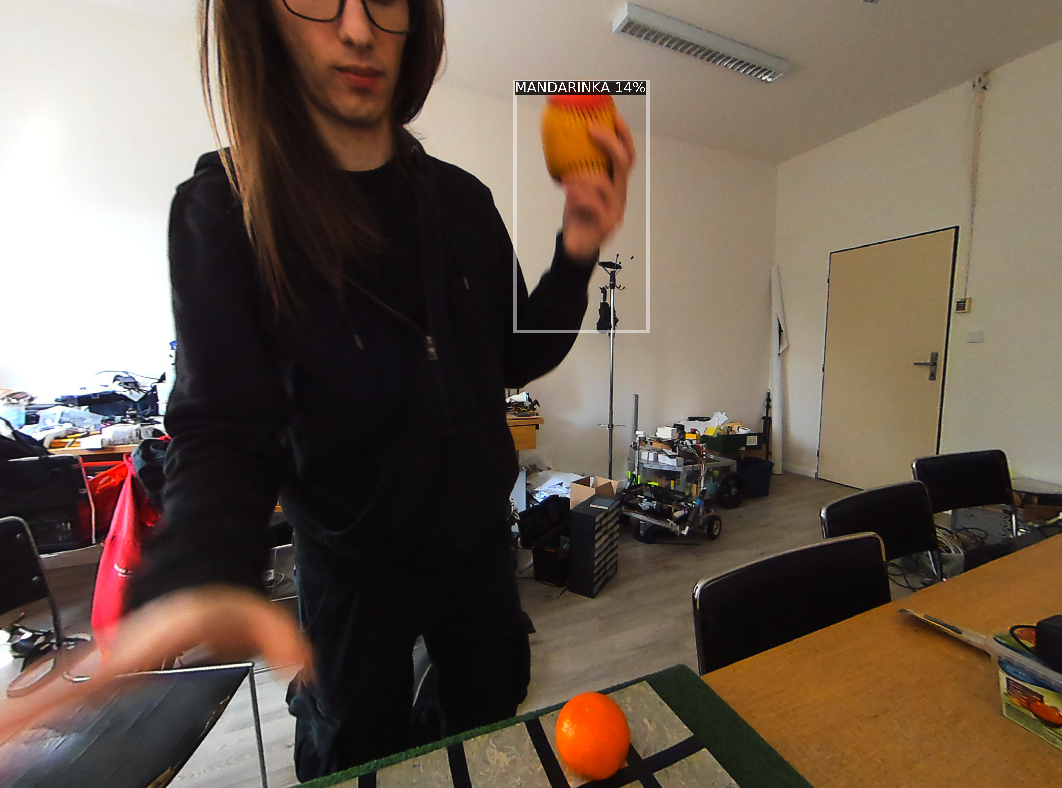
\includegraphics[width=\textwidth]{images/detections_screenshot_clean_wrong2.png}
\centering
\caption{Príklad neúspešných detekcií testovacích obrázkov z kamery robota NICO zbavených skreslenia.}
\label{fig:image705}
\end{figure}

\begin{table}[H]
\begin{tabular}{|l|c|c|c|}
\hline
\textbf{Trieda} & \textbf{mAP} & \textbf{AP50} & \textbf{AP75} \\
\hline
Mandarinka & 2.545 & 4.848 & 3.030 \\
\hline
\end{tabular}
\centering
\caption{Tabuľka presností na testovacích dátach pri detekcií mandarinky pomocou snímok z kamery robota NICO zbavených skreslenia.}
\label{tab:table701}
\end{table}

\begin{table}[H]
\begin{tabular}{|l|c|c|c|c|}
\hline
\textbf{Trieda} & \textbf{Počet obrázkov} & \textbf{Úspešné} & \textbf{Neúspešné} &  \textbf{Nedetegované}\\
\hline
Mandarinka & 20 & 2 & 7 & 18\\
\hline
\end{tabular}
\centering
\caption{Tabuľka jednoduchšej presnosti na testovacích dátach pri detekcií mandarinky pomocou snímok z kamery robota NICO zbavených skreslenia.}
\label{tab:table703}
\end{table}
